\section{Results}
\frame{\sectionpage}



\begin{frame}{Implementation}
    \begin{alertblock}{Stack}
        The implementation was done using the following frameworks
        \begin{enumerate}
            \item Python 3.7 (NumPy, Pandas and Scikit-Learn).
            \item MySQL 8.0.
            \item Jupyter Notebooks for experimentation.
            \item AWS EC2 for computing.
        \end{enumerate}
    \end{alertblock}
\end{frame}

\begin{frame}{Implementation}
    \begin{alertblock}{ML Parameters}

        The implementation was done using the following parameters
        \begin{enumerate}
            \item DT, SVM, RF and ET models.
            \item Statistical and Ergonomic Features.
            \item Jupyter Notebooks for experimentation.
            \item AWS EC2 for computing.
        \end{enumerate}
    \end{alertblock}
\end{frame}

\begin{frame}{Classification Results}
    \begin{figure}
        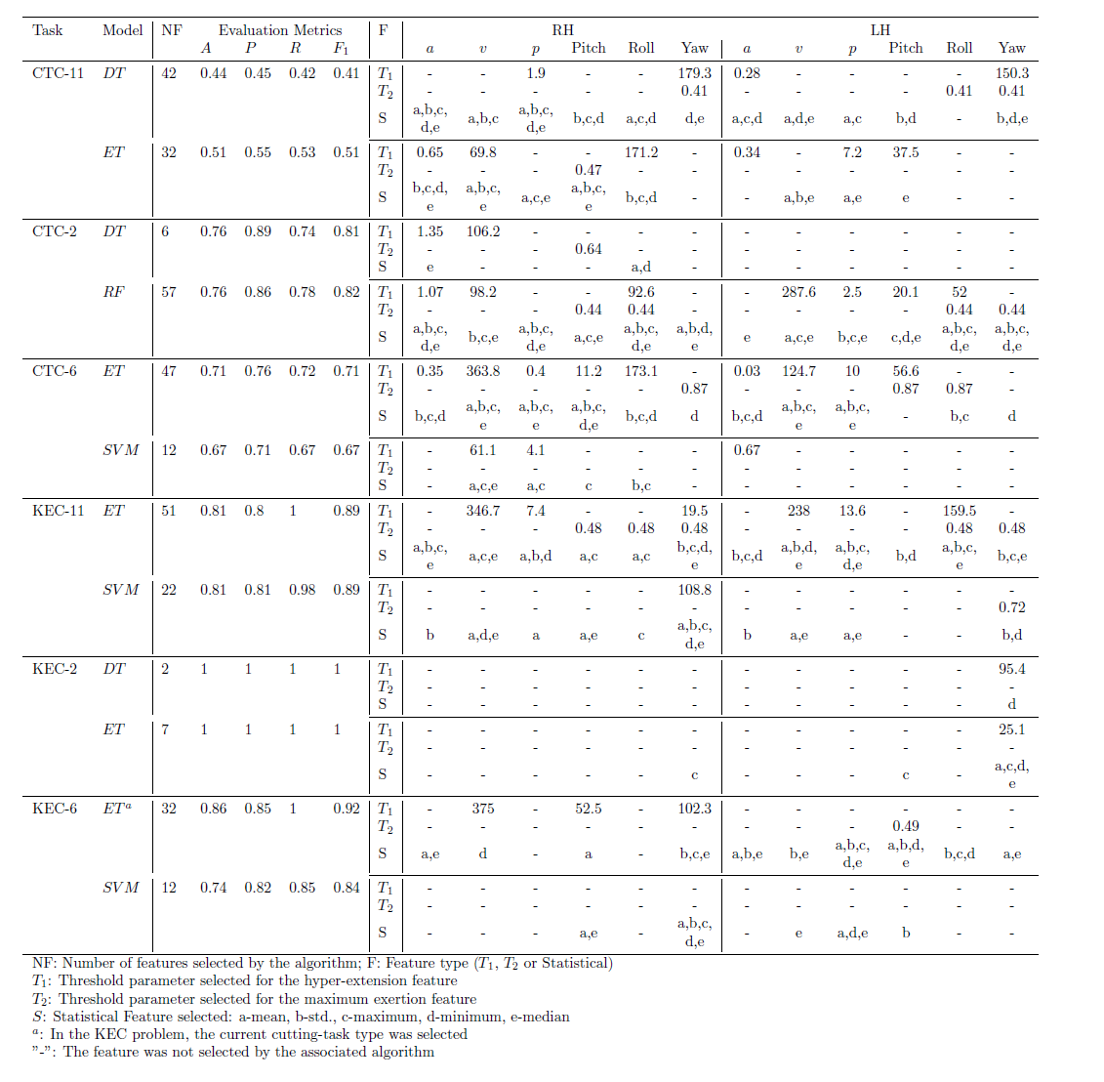
\includegraphics[scale=0.5]{img/results/classification_results_1.png}
    \end{figure}
\end{frame}

\begin{frame}{Classification Results}
    \begin{figure}
        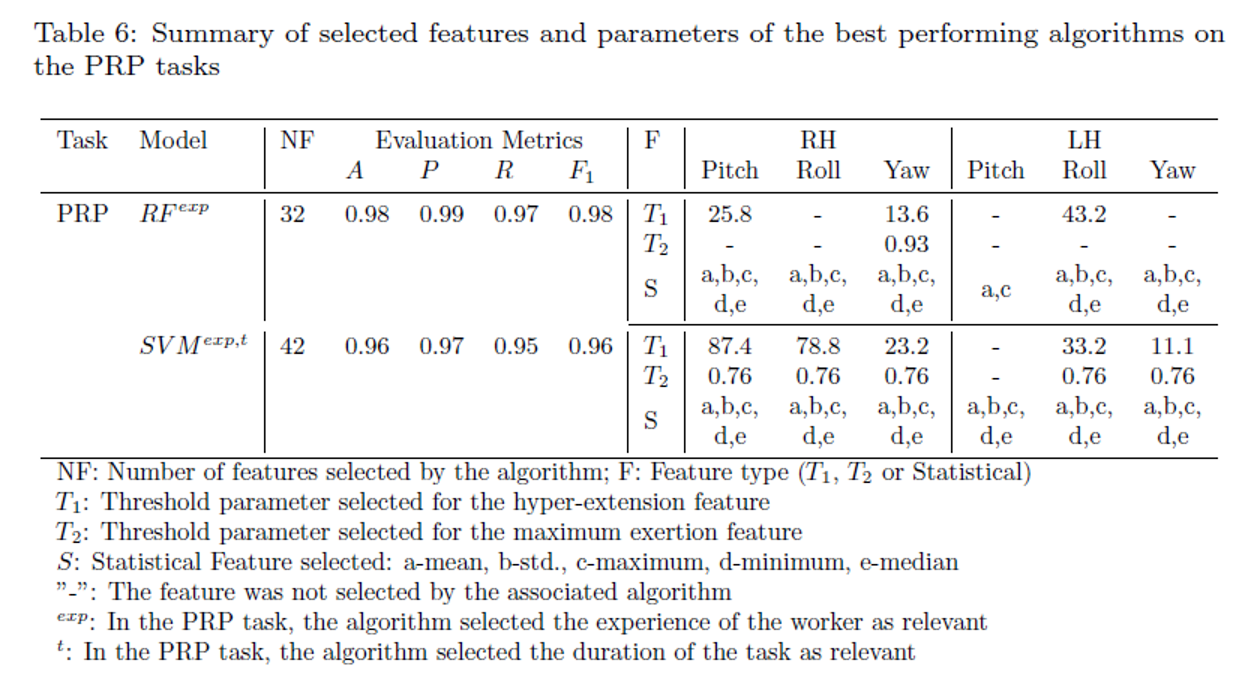
\includegraphics[scale=0.6]{img/results/classification_results_2.png}
    \end{figure}
\end{frame}

\begin{frame}{Classification Results}
    \begin{figure}
        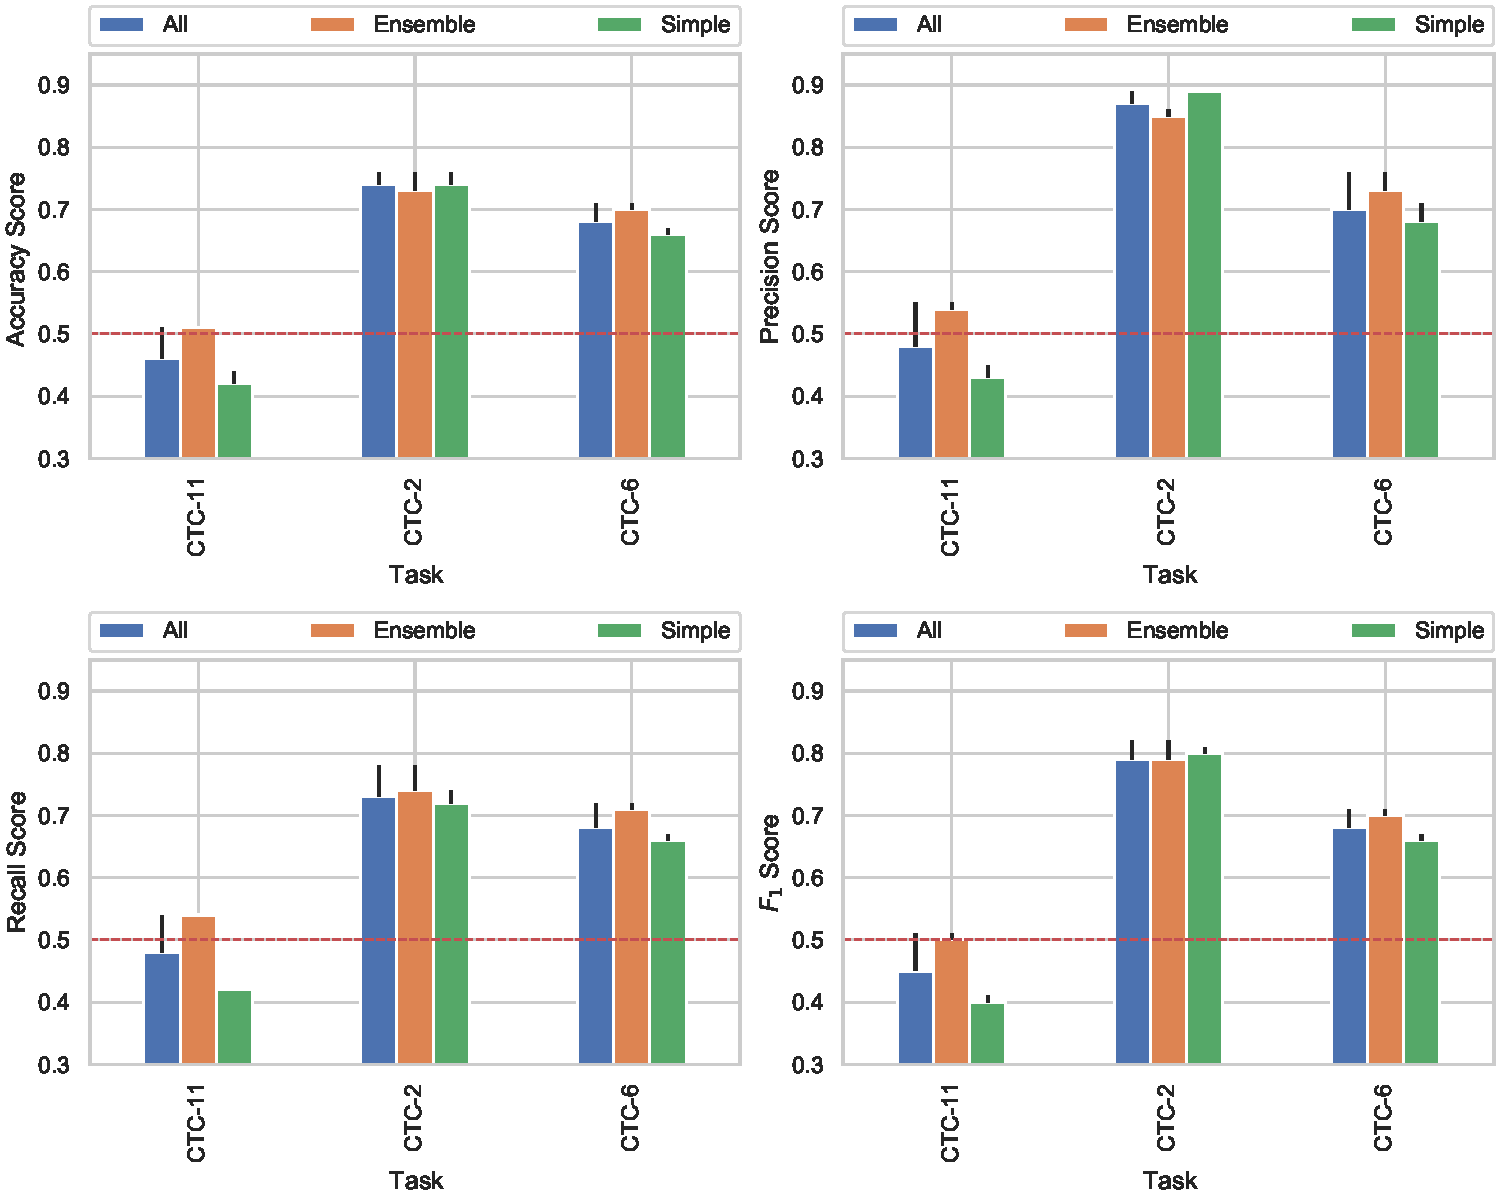
\includegraphics[scale=0.4]{img/results/CTC_summary.pdf}
    \end{figure}
\end{frame}

\begin{frame}{Classification Results}
    \begin{figure}
        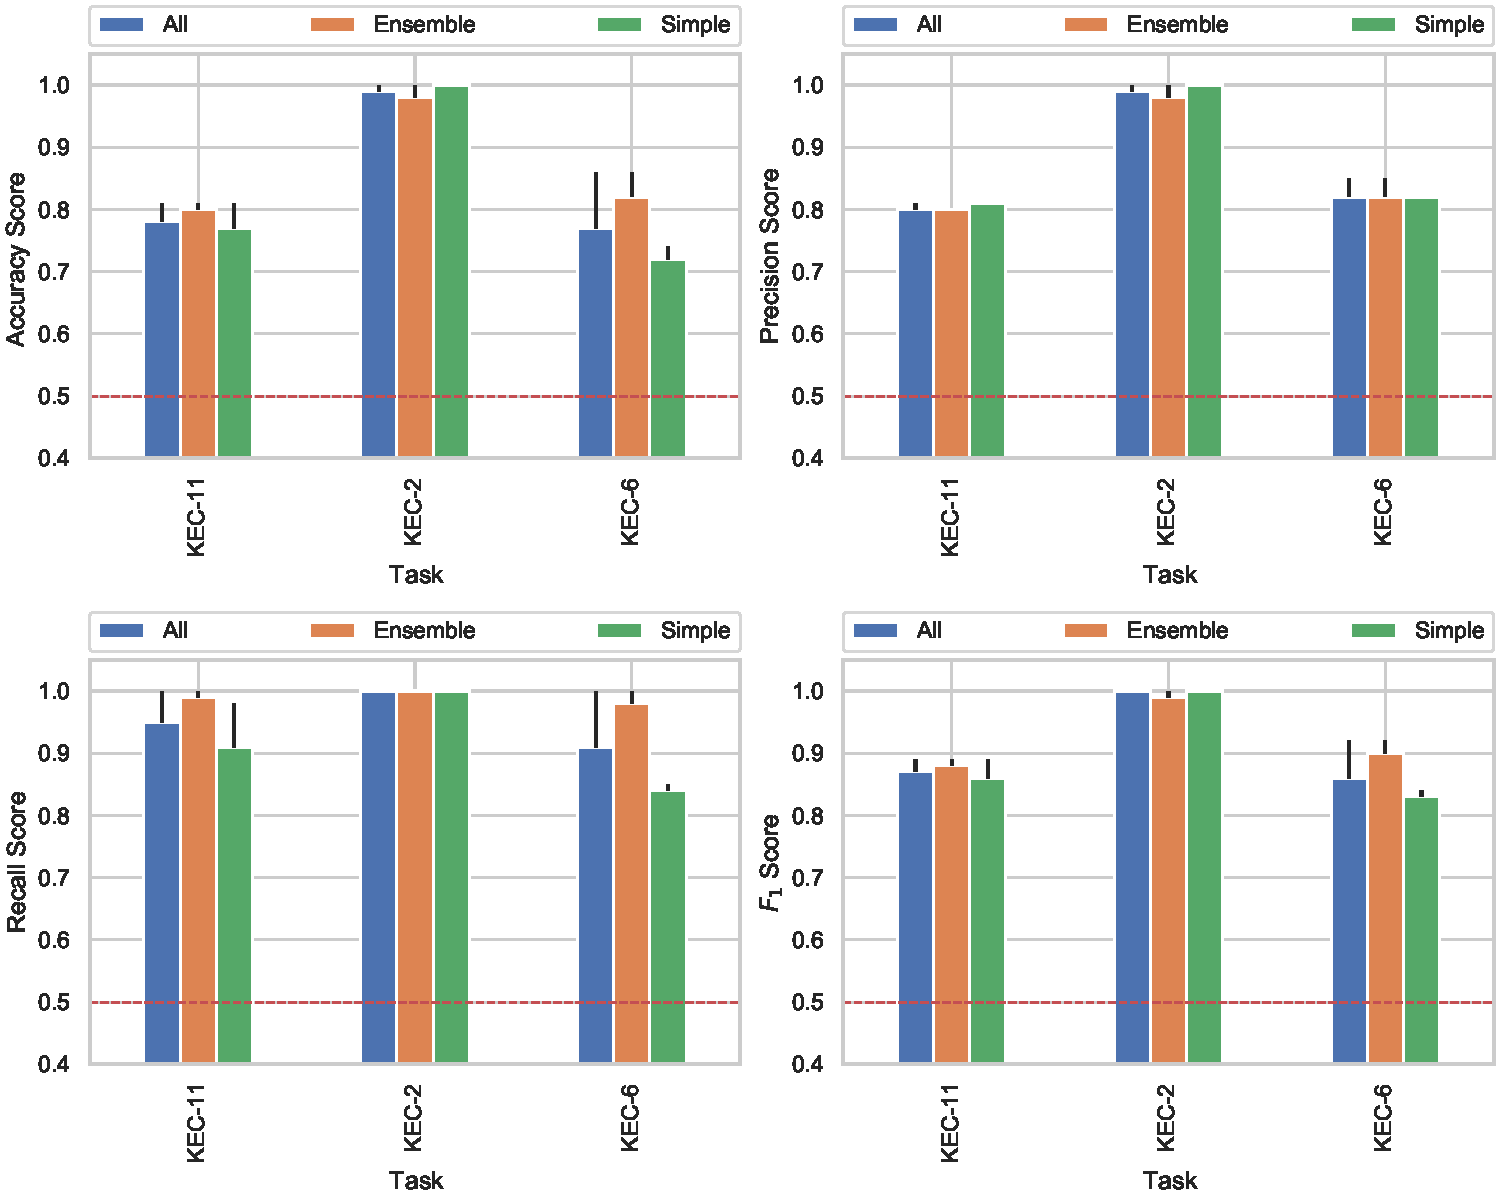
\includegraphics[scale=0.4]{img/results/KEC_summary.pdf}
    \end{figure}
\end{frame}

\begin{frame}{Effect of Knife Replacement}
    \begin{figure}
        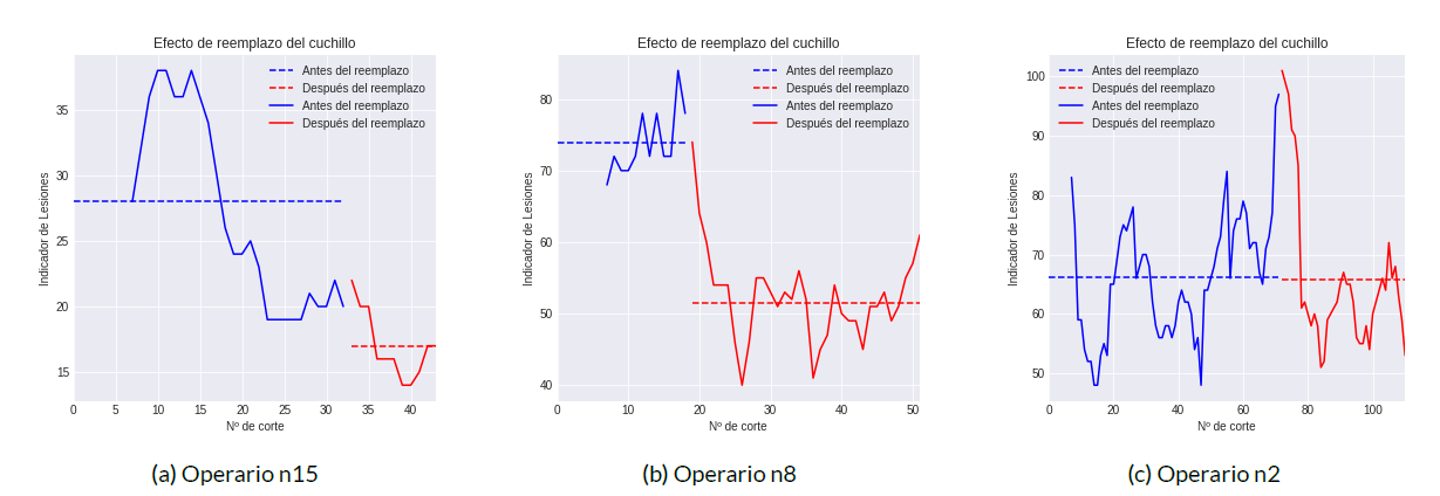
\includegraphics[scale=0.6]{img/results/knife_effect.png}
    \end{figure}
\end{frame}



\begin{frame}{Assessment of WRMSDs Risk}
    \begin{figure}
        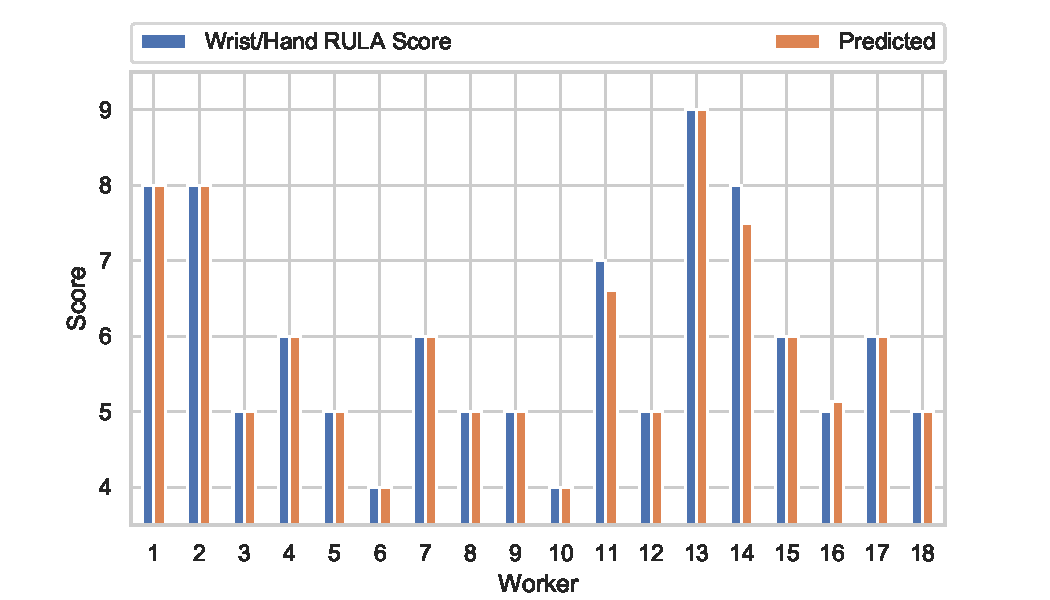
\includegraphics[scale=0.6]{img/results/rula_scores_predicted.pdf}
    \end{figure}
\end{frame}

\begin{frame}{Assessment of WRMSDs Risk}
    \begin{figure}
        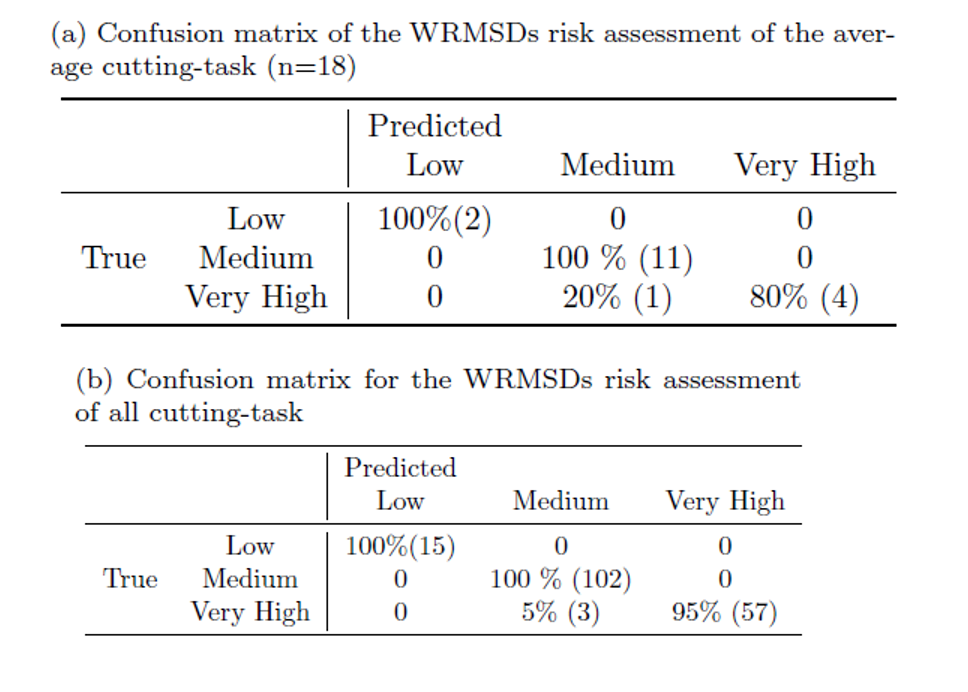
\includegraphics[scale=0.6]{img/results/decision_making.png}
    \end{figure}
\end{frame}